\section{Communication}

% https://mosquitto.org/man/mqtt-7.html <--- cool link
% https://docs.oasis-open.org/mqtt/mqtt/v5.0/mqtt-v5.0.pdf <-- also cool

Communication between the Raspberry Pi and the PC is handled using MQTT (Message Queuing Telemetry Transport) protocol. MQTT uses a publisher-subscriber model, where a publisher sends messages to a topic hosted on a broker, which then is sent to all subscribers (all components that need data from that topic) \cite{OASIS_MQTT5}.

MQTT messages consist of a fixed header, variable header and a payload. The fixed header contains information about the message type and flags, while the variable header contains topic name and packet identifier (if QoS $>$ 0).

Examples for variable header fields for different MQTT message types are shown in table \cref{tab:mqtt_packet_types}.

\begin{table}[htbp]
    \centering
    \begin{tabular}{l c c l}
        \toprule
        \textbf{Packet Type} & \textbf{Packet Type (Bits 7-4)} & \textbf{Hex} & \textbf{Purpose in the System} \\
        \midrule
        CONNECT  & 0001 & 0x10 & PC establishing connection to the broker. \\
        PUBLISH  & 0011 & 0x3\_ & \makecell[l]{Pi sends audio.\\PC sends commands.} \\
        SUBSCRIBE & 1000 & 0x8\_ & \makecell[l]{Pi subscribes to \texttt{mqtt\_vel} (velocity commands).\\PC subscribes to topics \texttt{I2S0} and \texttt{I2S1} for audio data.} \\
        PINGREQ  & 1100 & 0xC0 & All clients keep their connections alive. \\
        \bottomrule
    \end{tabular}
    \caption{MQTT control packet types used in the system and their values in the fixed header.}
    \label{tab:mqtt_packet_types}
\end{table}

The PUBLISH packet type is used for all application data. The last four bits of its fixed header are the DUP, RETAIN and the QoS (Quality of Service) level. 

A QoS of 0 means the message is delivered a maximum of one time, with no acknowledgment, so if it is lost it will not be retransmitted. 

A QoS of 1 means the message is delivered at least once, with acknowledgment, so if it is lost it will be retransmitted until acknowledged. 

A QoS of 2 means the message is delivered exactly once, with a four-step handshake to ensure no duplicates.

All data in the project, movement commands and audio data, are sent with a QoS of 1, to ensure they are received. 

The DUP flag is used for QOS 1 and 2 messages to indicate if the transmitted message is a duplicate of a previous attempt to send the same message. The RETAIN flag indicates if the broker should retain the last message sent to a topic, meaning the broker stores the last message, so if a new client subscribes to that topic, it immediately receives the last retained message.

The payload contains the actual data being transmitted. An example of an MQTT PUBLISH message structure is shown in table \cref{tab:mqtt_publish_example_bytes}.

\begin{table}[htbp]
    \centering
    \begin{tabular}{l l l}
        \toprule
        \textbf{Packet Section} & \textbf{Hex Bytes} & \textbf{Interpretation} \\
        \midrule
        Fixed Header & \texttt{0x30} & PUBLISH (0x3), QoS 1, DUP=0, RETAIN=0 \\
        Remaining Length & \texttt{0x1D} & 29 bytes to follow \\
        \midrule
        Variable Header & \texttt{0x00 0x07} & Topic Name Length: 7 bytes \\
        (Topic Name) & \texttt{0x63 0x6d 0x64 0x5f 0x76 0x65 0x6c} & Topic: cmd\_vel \\
        (Packet Identifier) & \texttt{0x00 0x19} & Packet ID: 25 \\
        \midrule
        Payload & \makecell[l]{\texttt{0x47 0x6f 0x20 \dots \space 0x74 0x65 0x72}} & Data: ``Go forward 1 meter" \\
        \bottomrule
    \end{tabular}
    \caption{Example byte breakdown of an MQTT PUBLISH packet (QoS 1, topic: ``cmd\_vel", payload: ``Go forward 1 meter").}
    \label{tab:mqtt_publish_example_bytes}
\end{table}

The maximum packet size is 256 MB for MQTT, which can be limited by modifying configurations for the chosen broker. In this project the mosquitto broker is used, which by default doesn't limit the maximum packet size \cite{mosquitto}. Mosquitto is the MQTT broker, which means it is the server that handles all messages being sent between clients. It ensures messages are sent to all subscribers of a topic when a publisher sends a message to that topic. Additionally, configurations like the QoS level can be set for each topic individually to ensure the desired reliability for each type of data.

In this project the python library paho-mqtt is used, which handles the low-level details of the MQTT protocol and parsing. Paho-mqtt ensures the components can connect to the mosquitto broker, which combined with the broker enables the transfer of data over TCP/IP, which in this project is done over WiFi \cite{paho-mqtt}.

\begin{figure}[H]
    \centering
    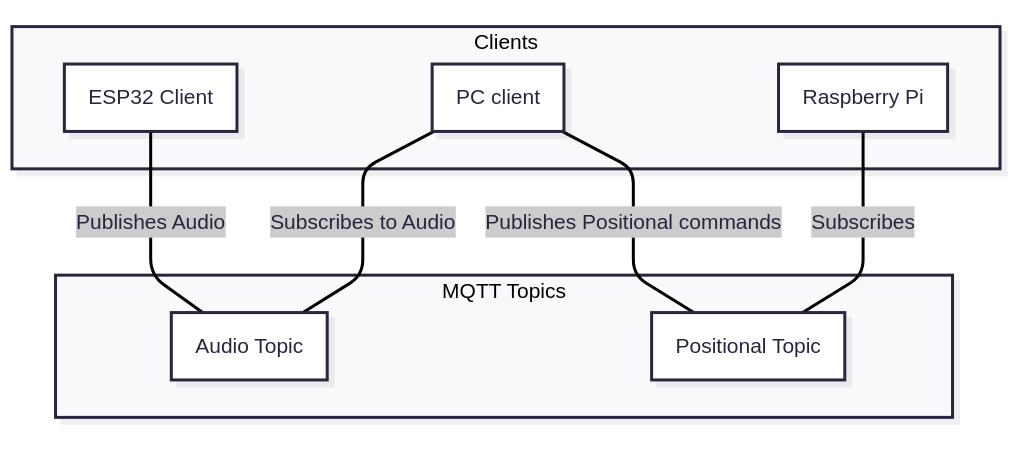
\includegraphics[width=0.8\linewidth]{Pictures/pubsub.png}
    \caption{MQTT topic setup for communication between the ESP32, PC, and Raspberry Pi.}
    \label{fig:mqtt_topic_setup}
\end{figure}